\hypertarget{_result_scene_state___start_8cpp}{}\section{C\+:/\+H\+A\+L/\+P\+G関係/03\+\_\+作成プログラム/03\+\_\+\+H\+A\+L授業/就職作品/\+Project/source/02\+\_\+\+Scene/\+Scenes/\+Result\+Scene/\+Result\+Scene\+State/\+Result\+Scene\+State\+\_\+\+Start/\+Result\+Scene\+State\+\_\+\+Start.cpp ファイル}
\label{_result_scene_state___start_8cpp}\index{C\+:/\+H\+A\+L/\+P\+G関係/03\+\_\+作成プログラム/03\+\_\+\+H\+A\+L授業/就職作品/\+Project/source/02\+\_\+\+Scene/\+Scenes/\+Result\+Scene/\+Result\+Scene\+State/\+Result\+Scene\+State\+\_\+\+Start/\+Result\+Scene\+State\+\_\+\+Start.\+cpp@{C\+:/\+H\+A\+L/\+P\+G関係/03\+\_\+作成プログラム/03\+\_\+\+H\+A\+L授業/就職作品/\+Project/source/02\+\_\+\+Scene/\+Scenes/\+Result\+Scene/\+Result\+Scene\+State/\+Result\+Scene\+State\+\_\+\+Start/\+Result\+Scene\+State\+\_\+\+Start.\+cpp}}


リザルトシーンステート(スタート)Class  


{\ttfamily \#include \char`\"{}Result\+Scene\+State\+\_\+\+Start.\+h\char`\"{}}\newline
{\ttfamily \#include \char`\"{}../../\+Result\+Scene.\+h\char`\"{}}\newline
{\ttfamily \#include $<$Scene\+Manager/\+Scene\+Manager.\+h$>$}\newline
{\ttfamily \#include $<$Scenes/\+Title\+Scene/\+Title\+Scene.\+h$>$}\newline
{\ttfamily \#include $<$Scenes/\+Title\+Scene/\+Title\+Scene\+State/\+Title\+Scene\+State\+\_\+\+Start/\+Title\+Scene\+State\+\_\+\+Start.\+h$>$}\newline
{\ttfamily \#include $<$Resource\+Manager\textbackslash{}\+Resource\+Manager.\+h$>$}\newline
{\ttfamily \#include $<$Safe\+Release/\+Safe\+Release.\+h$>$}\newline
{\ttfamily \#include $<$Convert\+To\+Frame\textbackslash{}\+Meter\+To\+Frame\textbackslash{}\+Meter\+To\+Frame.\+h$>$}\newline
{\ttfamily \#include $<$Keyboard\textbackslash{}\+Keyboard.\+h$>$}\newline
{\ttfamily \#include $<$2\+D/\+U\+I/\+Clear\+Logo/\+Clear\+Logo\+Factory/\+Clear\+Logo\+Factory.\+h$>$}\newline
{\ttfamily \#include $<$2\+D/\+U\+I/\+Failure\+Logo/\+Failure\+Logo\+Factory/\+Failure\+Logo\+Factory.\+h$>$}\newline
{\ttfamily \#include $<$2\+D\textbackslash{}\+U\+I\textbackslash{}\+Push\+Space\+Logo\textbackslash{}\+Push\+Space\+Logo\+Factory\textbackslash{}\+Push\+Space\+Logo\+Factory.\+h$>$}\newline
Result\+Scene\+State\+\_\+\+Start.\+cpp の依存先関係図\+:
\nopagebreak
\begin{figure}[H]
\begin{center}
\leavevmode
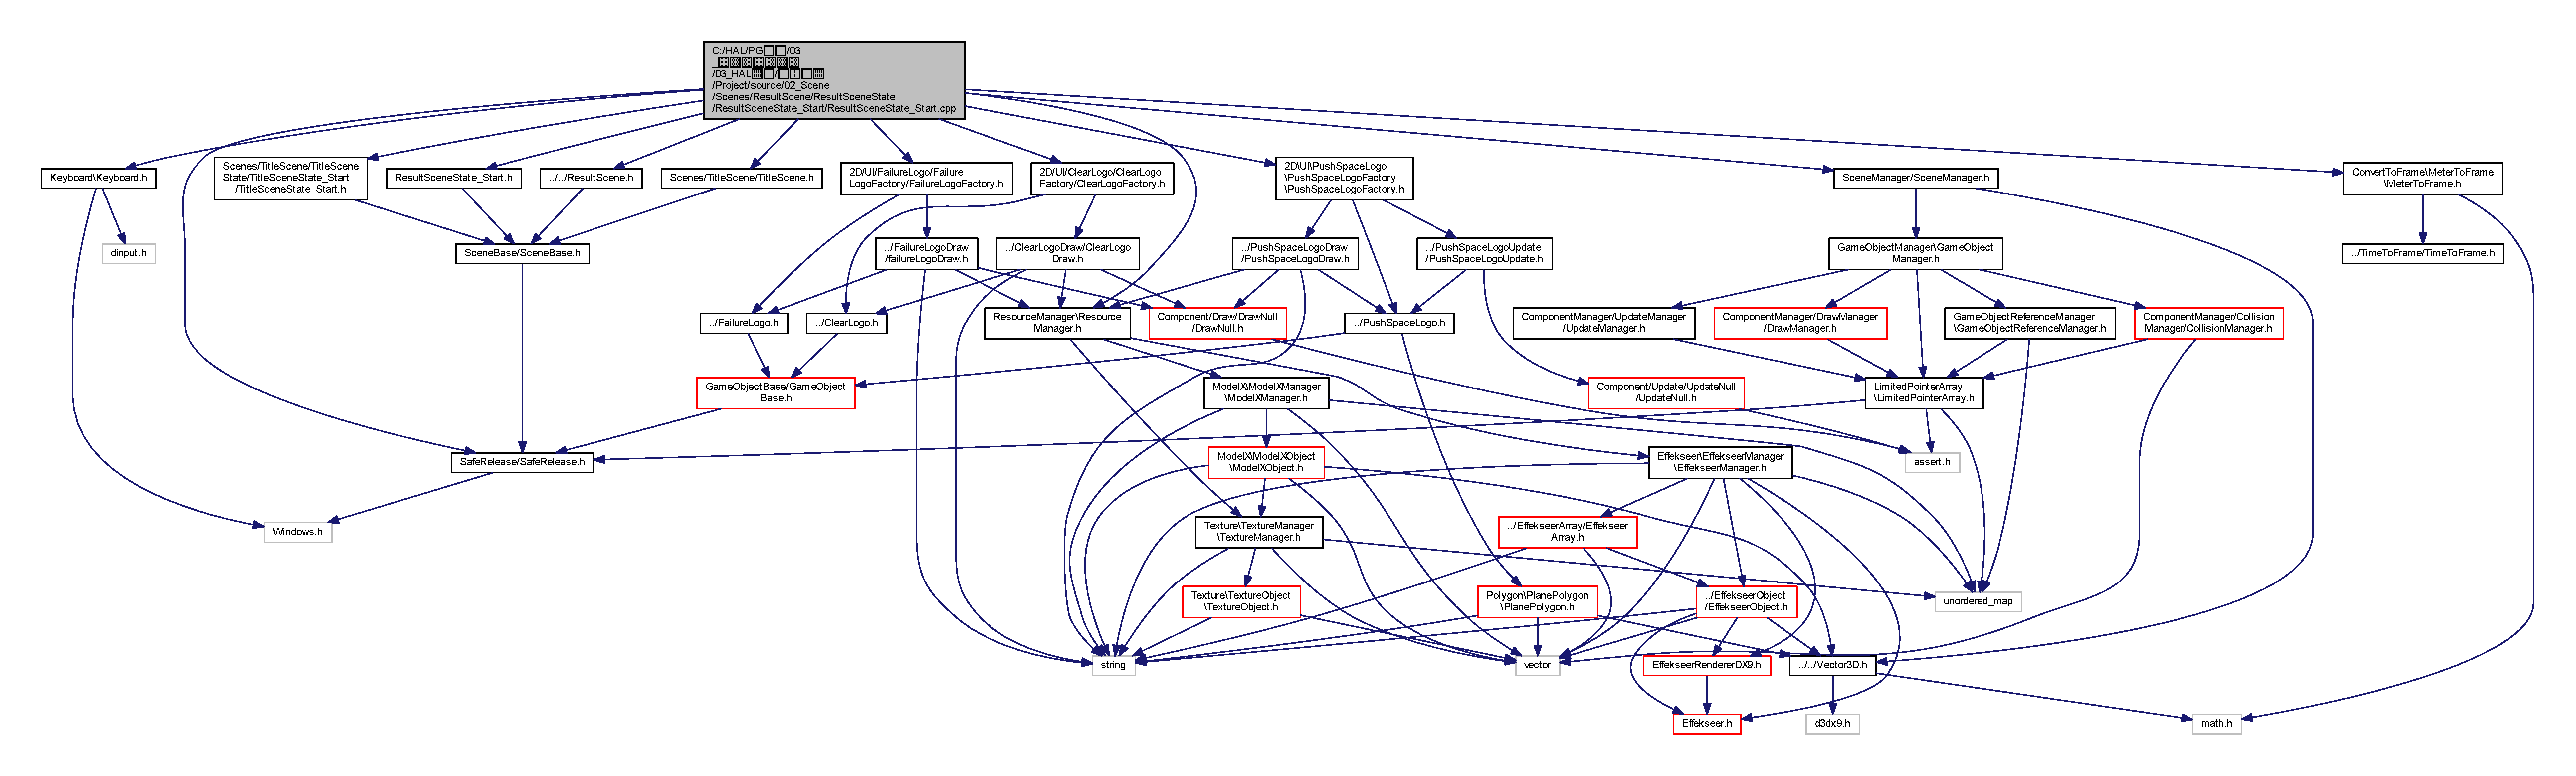
\includegraphics[width=350pt]{_result_scene_state___start_8cpp__incl}
\end{center}
\end{figure}


\subsection{詳解}
リザルトシーンステート(スタート)Class 

\begin{DoxyAuthor}{著者}
Kai Araki 
\end{DoxyAuthor}
\begin{DoxyDate}{日付}
2018/07/24 
\end{DoxyDate}
